\documentclass{article}
\usepackage[utf8]{inputenc}
\usepackage{MazzoleniNotation_rev3}
\usepackage{tabularx}
\usepackage{dirtytalk}
\usepackage{hyperref}
\usepackage{graphicx}   % for jpg images

\usepackage[margin=1in]{geometry}
\usepackage{xfrac}


\title{A practical guide for MAE 511}
\author{C. D. Yoder\\P. A. Sardeshmukh}
% \date{October 18$^{th}$ 2020}  % initial date, incomplete
% \date{December 26$^{th}$ 2020}  % rev1
\date{June 27$^{th}$ 2021}  % rev1

\begin{document}
\maketitle

% rotation matrices
\section{Frames}
\label{sec:frames}
Define a frame by a point and three orthogonal unit vectors. It is assumed there is an inertial frame $\bar{O}$ centered at Point O, and a relative frame $\bar{B}$ centered at Point B:
\begin{equation}
    \FrameDef{O}{O}
\end{equation}
\begin{equation}
    \FrameDef{B}{B}
\end{equation}

\section{Rotation matrices}
\label{sec:rotmat}
The rotation matrix $\RotateMat{B}{O}$, which rotates vectors from the $\bar{O}$ to the $\bar{B}$ frame, is termed the Direction Cosine Matrix:
\begin{equation}
    \RotateMat{B}{O} = \DirectCosMat
\end{equation}

\subsection{Euler angles}
\label{subsec:eulers}
Using three Euler angles $\theta$, $\phi$, $\psi$, each rotation about a single axis is defined as follows:
\begin{equation}
    \Rotate{\theta}{X} = \RotateMatX{\theta}
    \label{eq:x}
\end{equation}
\begin{equation}
    \Rotate{\phi}{Y} = \RotateMatY{\phi}
    \label{eq:y}
\end{equation}
\begin{equation}
    \Rotate{\psi}{Z} = \RotateMatZ{\psi}
    \label{eq:z}
\end{equation}
% 
The Direction Cosine Matrix is calculated by choosing a sequence of the three angles above. An example of several common sequences are defined (in Mazzoleni notation) as follows:
\subsubsection{XYZ sequence}
\begin{equation}
    \begin{split}
        \RotateMat{B}{O} & = \Rotate{\psi}{Z}\Rotate{\phi}{Y}\Rotate{\theta}{X} \\
         & =\RotateMatZ{\psi}\RotateMatY{\phi}\RotateMatX{\theta}
    \end{split}
\end{equation}
\subsubsection{YZX sequence}
\begin{equation}
    \begin{split}
        \RotateMat{B}{O} & = \Rotate{\theta}{X}\Rotate{\psi}{Z}\Rotate{\phi}{Y} \\
         & =\RotateMatX{\theta}\RotateMatZ{\psi}\RotateMatY{\phi}
    \end{split}
\end{equation}
\subsubsection{ZYX sequence}
\begin{equation}
    \begin{split}
        \RotateMat{B}{O} & = \Rotate{\theta}{X}\Rotate{\psi}{Y}\Rotate{\phi}{Z} \\
         & =\RotateMatX{\theta}\RotateMatZ{\psi}\RotateMatY{\phi}
    \end{split}
\end{equation}
Note that others define the $\RotateMat{O}{B}$ matrix instead, which uses both the transpose of Eqs. \ref{eq:x} - \ref{eq:z} and multiply in the order of the stated sequence\footnote{See \href{https://www.euclideanspace.com/maths/geometry/rotations/conversions/eulerToMatrix/index.htm}{https://www.euclideanspace.com/maths/geometry/rotations/conversions/eulerToMatrix/index.htm}}. 


\subsection{Quaternions}
\label{subsec:quats}
Instead of using three Euler angles to specify a rotation matrix, a quaternion, termed $\QuatDef{B}$ can be used:
\begin{equation}
    \RotateMat{B}{O} = \QuatBCO{}
\end{equation}
% 



\section{Angular velocity}
\label{sec:angvel}
Define the angular velocities of the $\bar{B}$ relative to the $\bar{O}$ frame as:
\begin{equation}
    \AngVel{O}{B}\cdot\UnitVec{i}{B} = \wX{B}{O}
    \label{eq:wx}
\end{equation}
%
\begin{equation}
    \AngVel{O}{B}\cdot\UnitVec{j}{B} = \wY{B}{O}
    \label{eq:wy}
\end{equation}
%
\begin{equation}
    \AngVel{O}{B}\cdot\UnitVec{k}{B} = \wZ{B}{O}
    \label{eq:wz}
\end{equation}
%
where $\RotateMatDot{O}{B}$ denotes the time derivative of the rotation matrix. Note that while the angular velocities are expressed in the relative frame (the $\bar{B}$ here), angles and quaternions (and their time derivatives) are frame-less. 
%
\subsection{Update relationships}
\label{subsec:updates}
The relationships in Eq. \ref{eq:wx}-\ref{eq:wz} are used to formulate the update relationships of the rotation matrices. For Euler angles, the update relationship depends on the sequence used. For quaternions, the update relationship can be expressed as:
\begin{equation}
    \QuatDot
    \label{eq:qd}
\end{equation}



\section{Position vectors}
\label{sec:posn}
The position vector of Point B with respect to Point O (or the position vector from O to B) is written:
\begin{equation}
    \PosVec{B}{O}
\end{equation}
%
Vector properties yields the following properties:
\begin{equation}
    \PosVec{B}{A} + \PosVec{A}{O} = \PosVec{B}{O}
    \label{eq:rbo}
\end{equation}
\begin{equation}
    \PosVec{O}{B} = -\PosVec{B}{O}
\end{equation}
% 
Finally, the center of mass of a rigid body with respect to a point is expressed as:
\begin{equation}
    \PosVec{CM}{B} = \frac{\sum_{i} m_i\PosVec{m_i}{B}}{\sum_{i} m_i} 
    \label{eq:rcm}
\end{equation}



\section{Transport theorems}
\label{sec:trans}
The first derivative transport theorem is defined as:
\begin{equation}
    \TransOne{O}{B}{\vec{A}}
    \label{eq:transone}
\end{equation}
The second derivative transport theorem is defined as:
\begin{equation}
    \TransTwo{O}{B}{\vec{A}}
    \label{eq:transtwo}
\end{equation}
where $\vec{A}$ denotes a vector. 


\section{Velocity vectors}
\label{sec:vel}
Using Eq. \ref{eq:transone}, the inertial velocity is expressed as:
\begin{equation}
    \VelVec{O}{B}{O} = \TransOne{O}{B}{\PosVec{B}{O}}
\end{equation}
Finding the inertial velocities of Eq. \ref{eq:rbo} and \ref{eq:rcm} yield:
\begin{equation}
    \VelVec{O}{B}{A} + \VelVec{O}{A}{O} = \VelVec{O}{B}{O}
    \label{eq:ovbo}
\end{equation}
\begin{equation}
    \VelVec{O}{CM}{B} = \frac{\sum_{i} m_i\VelVec{O}{m_i}{B}}{\sum_{i} m_i} 
    \label{eq:ovcmb}
\end{equation}




\section{Angular acceleration}
\label{sec:angaccl}
Using Eq. \ref{eq:transone} with the angular velocity vector yields:
\begin{equation}
    \AngAccl{O}{B} = \TransOne{O}{B}{\AngVel{O}{B}}
    \label{eq:angaccl}
\end{equation}
Note that the cross product $\Cross{\AngVel{O}{B}}{\AngVel{O}{B}}$ is zero. 




\section{Acceleration vectors}
\label{sec:accl}
Using Eq. \ref{eq:transtwo}, the inertial acceleration is expressed as:
\begin{equation}
    \AcclVec{O}{B}{O} = \TransTwo{O}{B}{\PosVec{B}{O}}
\end{equation}
Finding the inertial accelerations of Eq. \ref{eq:rbo} and \ref{eq:rcm} yield:
\begin{equation}
    \AcclVec{O}{B}{A} + \AcclVec{O}{A}{O} = \AcclVec{O}{B}{O}
    \label{eq:oabo}
\end{equation}
\begin{equation}
    \AcclVec{O}{CM}{B} = \frac{\sum_{i} m_i\AcclVec{O}{m_i}{B}}{\sum_{i} m_i} 
    \label{eq:oacmb}
\end{equation}




\section{Angular momentum}
\label{sec:angmom}
The angular momentum of a system of particle is defined as:
\begin{equation}
    \AngMom{F}{Q}{A} = \sum_{i} \AngMom{F}{Q}{\sfrac{m_i}{A}} = \sum_{i} \Big( \Cross{\PosVec{m_i}{A}}{m_i\VelVec{F}{m_i}{Q}} \Big)
    \label{eq:angmom}
\end{equation}
Using Eq. \ref{eq:rcm}, the angular momentum of a system of particles about the center of mass is:
\begin{equation}
    \AngMom{O}{Q}{A} = m_{sys} \Cross{\PosVec{CM}{A}}{\VelVec{O}{CM}{Q}}
    \label{eq:ohqa1}
\end{equation}
Using Eq. \ref{eq:rbo}, the angular momentum of a system of particles including a generic Point P is:
\begin{equation}
    \AngMom{O}{Q}{A} = \Cross{\PosVec{CM}{A}}{m_{sys}\VelVec{O}{P}{Q}} + \Cross{\PosVec{P}{A}}{m_{sys}\VelVec{O}{CM}{P}} + \AngMom{O}{P}{P} 
    \label{eq:ohqa2}
\end{equation}
Expanding $\AngMom{O}{P}{P}$ by it's definition and using the definition of an inertia tensor yields:
\begin{equation}
    \AngMom{O}{Q}{A} = \Cross{\PosVec{CM}{A}}{m_{sys}\VelVec{O}{P}{Q}} + \Cross{\PosVec{P}{A}}{m_{sys}\VelVec{O}{CM}{P}} + \AngMom{B}{P}{P} + \Inert{P}\cdot\AngVel{O}{B}
    \label{eq:ohqa3}
\end{equation}
For a rigid body, $\AngMom{B}{P}{P} = \sum_{i} \Big( \Cross{\PosVec{m_i}{P}}{m_i\vec{0}} \Big) = 0$, resulting in:
\begin{equation}
    \AngMom{O}{Q}{A} = \Cross{\PosVec{CM}{A}}{m_{sys}\VelVec{O}{P}{Q}} + \Cross{\PosVec{P}{A}}{m_{sys}\VelVec{O}{CM}{P}} + \Inert{P}\cdot\AngVel{O}{B}
    \label{eq:ohqa4}
\end{equation}
For a system of $n$ rigid bodies denoted by $m_j$:  
\begin{equation}
    \AngMom{O}{Q}{A}\vert_{sys} = \sum_{j}^{n} \AngMom{O}{Q}{A}\vert_{m_j}
    \label{eq:ohqa5}
\end{equation}
where:
\begin{enumerate}
    \item $\bar{O}$ denotes the velocities are with respect to the $\bar{O}$ frame
    \item Point Q is a point which either (1) is stationary, or (2) has a constant velocity relative to an inertial frame (easiest to set Point Q to Point O)
    \item Point CM is the center of mass of the cluster of points
    \item $m_{sys}$ is the total mass of all particles in the system
    \item Point P is some alternate point of interest (e.g. geometric center of a tumbleweed rover, nose of an aircraft, etc)
    \item $\AngMom{B}{P}{P} = \sum_{i} \Cross{\PosVec{m_i}{P}}{m_i\VelVec{B}{m_i}{P}}$
    \item $\Inert{P}\cdot\AngVel{O}{B} = \sum_{i} \Cross{\PosVec{m_i}{P}}{m_i\Big(\Cross{\AngVel{O}{B}}{\PosVec{m_i}{P}}}\Big)$
    \item $\Inert{P}$ can be a tensor with elements which are functions of time, angles, etc., however it is best to choose Point P such that $\Inert{P}$ is constant, if possible
    \item Point P can be different for each rigid body $m_j$ in a single system when calculating $\AngMom{O}{Q}{A}\vert_{sys}$
\end{enumerate}



\section{Forces}
From Newton's second law:
\begin{equation}
    \Fext = m\AcclVec{O}{CM}{O}
    \label{eq:newton2}
\end{equation}
Applying Eq. \ref{eq:oabo} and Eq. \ref{eq:oacmb}:
\begin{equation}
    \Fext = m\Big( \AcclVec{O}{CM}{B} + \AcclVec{O}{B}{O} \Big)
    \label{eq:feqma}
\end{equation}



\section{Moments}
Taking the derivative of angular momentum (and recognizing the definition of torque) yields:
\begin{equation}
    \FrameDeriv{O}{t}{\AngMom{O}{Q}{A}} = \Text[A] - \Big( \Cross{\VelVec{O}{A}{O}}{m_{sys}\VelVec{O}{CM}{O}} \Big)
    \label{eq:sumtorq}
\end{equation}



% ----------------------------------------------------------
\newpage
\section*{Appendix: Determining rotation angles in a sequence}
Sometimes, there is a need to write the rotation matrix between two frames which are fixed with respect to each other (e.g. stability vs body frame of an aircraft). Using Mazzoleni notation:
\begin{enumerate}
    \item Graphically draw the second frame relative to the first frame.
    \item Pick a rotation scheme. 
    \item In the backwards order of the scheme, rotate the first frame to the second using only angles about the subsequent frames. 
    \item Multiply the individual matrices in the same order to form the $\RotateMat{B}{O}$ matrix. 
\end{enumerate}
% 
Consider the following example:
\begin{enumerate}
    \item Draw the frames:
    \begin{figure}[h]
        \centering
        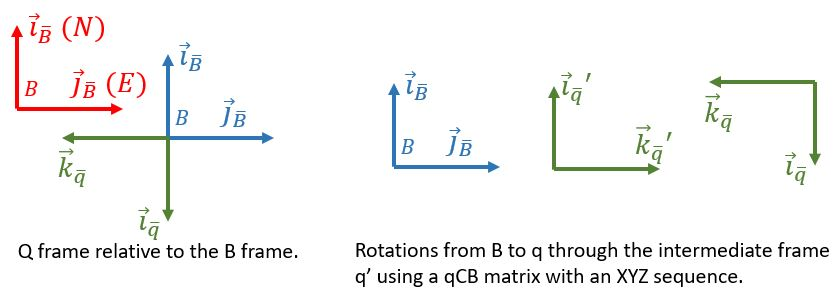
\includegraphics{pics/Capture.JPG}
        \label{fig:ex1}
    \end{figure}
    \item Rotation scheme: XYZ
    \item Find angles:
    \begin{enumerate}
        \item Rotate $-\pi/2$ about X (B frame)
        \item Rotate $\pi$ about Y (q' frame)
        \item Rotate $0$ about Z
    \end{enumerate}
    \item Make the $\RotateMat{q}{B}$ matrix:
    \begin{equation}
        \begin{split}
            \RotateMat{q}{B} & =\RotateMatZ{0}\RotateMatY{\pi}\RotateMatX{-\pi/2} \\
            & = \GenMat{-1}{0}{0}{0}{0}{-1}{0}{-1}{0}
        \end{split}
    \end{equation}
\end{enumerate}
% 
A simple check is to express the unit vectors of the $\bar{B}$ frame in the $\bar{q}$ frame. Thus, $\Frame{\UnitVec{i}{B}}{q}$, $\Frame{\UnitVec{j}{B}}{q}$, and $\Frame{\UnitVec{k}{B}}{q}$ are found to be $\VecExpressH{q}{-1}{0}{0}$, $\VecExpressH{q}{0}{0}{-1}$, and  $\VecExpressH{q}{0}{-1}{0}$, which is verified by inspection. 




% ----------------------------------------------------------
\newpage
\section*{Appendix: Finding the rotation matrix from two vectors}
For navigation applications, it is often required to find the rotation matrix between an inertial frame and a body frame. This can be done using two vectors known (or modelled) in the inertial frame and measured in the body frame. For this example, consider the two vectors $\vec{s}$ and $\vec{m}$. First, define both vectors as unit vectors in the $\bar{B}$ and the $\bar{O}$ frames:
\begin{equation}
    \hat{s}_B = \Frame{\vec{s}/||\vec{s}||_2}{B}
\end{equation}
\begin{equation}
    \hat{s}_O = \Frame{\vec{s}/||\vec{s}||_2}{O}
\end{equation}
\begin{equation}
    \hat{m}_B = \Frame{\vec{m}/||\vec{m}||_2}{B}
\end{equation}
\begin{equation}
    \hat{m}_O = \Frame{\vec{m}/||\vec{m}||_2}{O}
\end{equation}

Second, construct the first of two required basis vectors:
\begin{equation}
    \hat{t}_{1_B} = \hat{s}_B
\end{equation}
\begin{equation}
    \hat{t}_{1_O} = \hat{s}_O
\end{equation}

Next, define a second vector as the cross product of $\hat{s}$ and $\hat{m}$:
\begin{equation}
    \hat{t}_{2_B} = (\Cross{\hat{s}_B}{\hat{m}_B})/||\Cross{\hat{s}_B}{\hat{m}_B}||_2
\end{equation}
\begin{equation}
    \hat{t}_{2_O} = (\Cross{\hat{s}_O}{\hat{m}_O})/||\Cross{\hat{s}_O}{\hat{m}_O}||_2
\end{equation}

Fourth, define the third basis vector orthogonal to the first two vectors:
\begin{equation}
    \hat{t}_{3_B} = \Cross{\hat{t}_{1_B}}{\hat{t}_{2_B}}
\end{equation}
\begin{equation}
    \hat{t}_{3_O} = \Cross{\hat{t}_{1_O}}{\hat{t}_{2_O}}
\end{equation}

Finally, construct the \RotateMat{B}{O} matrix as follows:
\begin{equation}
    \RotateMat{B}{O} = [\hat{t}_{1_B}, \hat{t}_{2_B}, \hat{t}_{3_B}][\hat{t}_{1_O}, \hat{t}_{2_O}, \hat{t}_{3_O}]^T
\end{equation}

Note: this derivation is not originally from EMSSL. For credit, please refer to \url{http://www.dept.aoe.vt.edu/~cdhall/courses/aoe4140/attde.pdf}. 




% ----------------------------------------------------------
\newpage
\section*{Appendix: Equations of motion}
Consider a single rigid body embedded with a relative frame \FrameDef{B}{B} moving relative to an inertial frame \FrameDef{O}{B}. The states of the problem are given by:
\begin{equation}
    \vec{x} = \{\PosVec{B}{O}, \VelVec{B}{B}{O}, \vec{a}, \AngVel{O}{B}\}^{T}
\end{equation}
where:
\begin{itemize}
    \item $\PosVec{B}{O} = [x_B, y_B, z_B]$
    \item $\VelVec{B}{B}{O} = [u_B, v_B, w_B]$
    \item $\vec{a} = [\theta, \phi, \psi]$ for Euler angles
    \item $\vec{a} = [q_0, q_1, q_2, q_3]$ for Quaternions
    \item $\AngVel{O}{B} = [p_B, q_B, r_B]$
\end{itemize}
The state derivatives of the problem are:
\begin{equation}
    \dot{\vec{x}} = \{\VelVec{B}{B}{O}, \AcclVec{B}{B}{O}, \dot{\vec{a}}, \AngAccl{O}{B}\}^{T}
\end{equation}
where:
\begin{itemize}
    \item $\AcclVec{B}{B}{O} = [\dot{u_B}, \dot{v_B}, \dot{w_B}]$
    \item $\dot{\vec{a}} = [\dot{\theta}, \dot{\phi}, \dot{\psi}]$ for Euler angles
    \item $\dot{\vec{a}} = [\dot{q_0}, \dot{q_1}, \dot{q_2}, \dot{q_3}]$ for Quaternions
    \item $\AngAccl{O}{B} = [\dot{p_B}, \dot{q_B}, \dot{r_B}]$
\end{itemize}
Using Eq. \ref{eq:qd} (or Eq. \ref{eq:wx}-\ref{eq:wz}), \ref{eq:feqma}, and \ref{eq:sumtorq}, the state derivatives can be expressed as functions of time and the states:
\begin{equation}
    \dot{\vec{x}} = f(t, \vec{x})
    \label{eq:xdofx}
\end{equation}
This form is the most useful form of the body's equations of motion. 



% ----------------------------------------------------------
\newpage
\section*{Appendix: Integration of equations of motion}
To integrate the equations of motion:
\begin{enumerate}
    \item Write the equations of motion in the form in Eq. \ref{eq:xdofx}
    \item The first scheme to be used should be a Range-Kutta 4(5) integration scheme, which is available on most modern computing packages
\end{enumerate}
Note that:
\begin{itemize}
    \item All state variables need not be expressed in the same frame for integration. However, the equations must be valid (e.g. all vectors must be rotated into a single frame before solving an equation). 
    \item If the equations are said to be stiff or numerically ill-conditioned, alternate solvers should be used. 
\end{itemize}




% ----------------------------------------------------------
\newpage
\section*{Appendix: Energy methods}
% ----------------------------------------------------------
\newpage
\section*{Appendix: Kane's method}
% ----------------------------------------------------------
\newpage
\section*{Appendix: Example problem - Slipping v rolling}
% ----------------------------------------------------------
\newpage
\section*{Appendix: Bead models}
% ----------------------------------------------------------
\newpage
\section*{Appendix: Added mass effect}
% ----------------------------------------------------------
\newpage
\section*{Appendix: Derivation using MATLAB}
% ----------------------------------------------------------
\newpage
\section*{Appendix: Tips for solving equations}
% ----------------------------------------------------------
\newpage
\section*{Appendix: Example problem - Yo-Yo de-spin problem}
\url{https://en.wikipedia.org/wiki/Yo-yo_de-spin}


% ----------------------------------------------------------
\end{document}
